\input{header_beamer}
\usepackage{etex}
%\include{macros}
%\documentclass[usenames,dvipsnames]{beamer}
%\usepackage{beamerthemesplit}
%\usepackage{graphics}
%\usepackage{amsmath}
%\usepackage{rotating}
%\usepackage{array}
%\usepackage{nth}
\usepackage{xcolor}
\usepackage{textcomp}
\input{matlab_setup}

\usepackage{tabularx}
\usepackage{picins}
\usepackage{tikz}
\usepackage{changepage}
\usepackage{wasysym} % for smileys
\usepackage{fp}

\usetikzlibrary{shapes.geometric,arrows,chains,matrix,positioning,scopes,calc}
\tikzstyle{mybox} = [draw=white, rectangle]

\definecolor{camlightblue}{rgb}{0.601 , 0.8, 1}
\definecolor{camdarkblue}{rgb}{0, 0.203, 0.402}
\definecolor{camred}{rgb}{1, 0.203, 0}
\definecolor{camyellow}{rgb}{1, 0.8, 0}
\definecolor{lightblue}{rgb}{0, 0, 0.80}
\definecolor{white}{rgb}{1, 1, 1}
\definecolor{whiteblue}{rgb}{0.80, 0.80, 1}
\definecolor{mydarkblue}{rgb}{0.00,0.08,0.45}

\newcolumntype{x}[1]{>{\centering\arraybackslash\hspace{0pt}}m{#1}}
\newcommand{\tabbox}[1]{#1}

% Deep net notation
\def\onefeat{h}
\def\feat{\vh}
\newcommand{\netweights}{w}
\newcommand{\vnetweights}{\vw}
\newcommand{\mnetweights}{\vW}


%%%%%%%%%%%%%%%%%%%%%%%%%%%%%%%%%%%%%%%%%%%
%
% Some look and feel definitions
%
%%%%%%%%%%%%%%%%%%%%%%%%%%%%%%%%%%%%%%%%%%%

\setlength{\columnsep}{0.03\textwidth}
\setlength{\columnseprule}{0.0018\textwidth}
\setlength{\parindent}{0.0cm}

%\include{macros}
\usepackage{preamble}
\hypersetup{colorlinks=true,citecolor=blue}
%\pdfmapfile{+sansmathaccent.map}

\title{Visualizing Priors on Deep Networks}


\author{
\hspace{-1cm}
\includegraphics[height=0.2\textwidth, trim=20mm 25mm 0mm 25mm, clip]{figures/david2}
\qquad\quad
\includegraphics[height=0.2\textwidth]{figures/rippel2}
\qquad\quad
\includegraphics[height=0.2\textwidth]{figures/adams}
\qquad\quad
\includegraphics[height=0.2\textwidth]{figures/zg2}
\hspace{-1cm}
\\
\hspace{-0.9cm}
David Duvenaud, Oren Rippel, Ryan Adams, Zoubin Ghahramani
\hspace{-0.9cm}
}

\institute{
\includegraphics[width=0.12\textwidth]{badges/cam-crest-and-text}
\hspace{3cm}
\includegraphics[width=0.2\textwidth]{badges/harvard}
}
%\date{}


\begin{document}

% Macros for inluding series of images.
%\newcommand{\onedsamplepic}[1]{
%\includegraphics[width=0.7\columnwidth]{figures/1d_samples/latent_seed_0_1d_large/layer-#1}}

\newcommand{\onedsamplepic}[1]{{
\begin{tabular}{cc}
\raisebox{2.5cm}{$f(x)$} & \includegraphics[width=0.6\columnwidth,clip,trim=10mm 5mm 4mm 7mm]{figures/1d_samples/latent_seed_0_1d_large/layer-#1} \\
 & $x$
 \end{tabular}}}


\newcommand{\onedsamplepiccon}[1]{{
%\includegraphics[width=0.7\columnwidth]{figures/1d_samples/latent_seed_0_1d_large_connected/layer-#1}
%\includegraphics[width=0.67\columnwidth]{figures/seed-0-map/latent_coord_map_layer_#1}%
%}
\begin{tabular}{cc}
\raisebox{2.5cm}{$f(x)$} & \includegraphics[width=0.6\columnwidth,clip,trim=10mm 5mm 4mm 7mm]{figures/1d_samples/latent_seed_0_1d_large_connected/layer-#1} \\
 & $x$
 \end{tabular}}}
 
 

\newcommand{\gpdrawbox}[1]{
\setlength\fboxsep{0pt}
\fbox{
\includegraphics[width=0.67\columnwidth]{figures/deep_draws/deep_gp_sample_layer_#1}
}}
\newcommand{\mappic}[1]{
%\includegraphics[width=0.6\columnwidth]{figures/map/latent_coord_map_layer_#1}
\includegraphics[width=0.67\columnwidth]{figures/seed-0-map/latent_coord_map_layer_#1}
} 
\newcommand{\mappiccon}[1]{
\includegraphics[width=0.67\columnwidth]{figures/seed-0-map-connected/latent_coord_map_layer_#1}
%\includegraphics[width=0.6\columnwidth]{figures/map_connected/latent_coord_map_layer_#1}
}



\newcommand{\gpdrawboxcon}[1]{
\setlength\fboxsep{0pt}
\fbox{
\includegraphics[width=0.67\columnwidth]{figures/deep_draws_connected/deep_sample_connected_layer#1}%
}}%



%\setbeamertemplate{background canvas}{\begin{tikzpicture}\node[opacity=.1]{\includegraphics [width=\paperwidth]{figures/map_connected/latent_coord_map_layer_40}};\end{tikzpicture}}
\setbeamertemplate{background canvas}{\centering 
\begin{tikzpicture}\node[opacity=.2]{\centering \includegraphics [width=\paperwidth]{figures/deep_gp_movie_486}};\end{tikzpicture}}



\frame[plain] {
\titlepage
}

\setbeamertemplate{background canvas}{}




\frame[plain]{
\frametitle{What this talk is about}
\begin{itemize}
%	\item Deep neural networks define functions: $\vy = \vf(\vx)$
%	\item A prior on deep nets defines a prior on functions.
%	\item Closely related to constructing priors
	\item Neural nets require lots of design choices, implications hard to understand.
	\item Why not just sample from priors on deep nets?
	\item Might help understand them without reference to a specific dataset, loss function, or training method.
	\item We'll visualize and analyze sampled neural nets:
\begin{tabular}{cccc}
%\includegraphics[width=0.17\columnwidth,clip,trim=10mm 5mm 7.5mm 6.5mm]{figures/1d_samples/latent_seed_0_1d_large/layer-5}
%&
{\setlength\fboxsep{0pt}
\fbox{\includegraphics[width=0.17\columnwidth]{figures/deep_draws/deep_gp_sample_layer_5}
}}
&
\includegraphics[width=0.17\columnwidth]{figures/seed-0-map/latent_coord_map_layer_6}
&
{\setlength\fboxsep{0pt}
\fbox{\includegraphics[width=0.17\columnwidth]{figures/deep_draws_connected/deep_sample_connected_layer3}
}}
&
\includegraphics[width=0.17\columnwidth]{figures/seed-0-map-connected/latent_coord_map_layer_6}
%&
%\includegraphics[width=0.17\columnwidth]{figures/seed-0-map-connected/latent_coord_map_layer_6}
%&
%\includegraphics[width=0.17\columnwidth]{figures/1d_samples/latent_seed_0_1d_large_connected/layer-6}
%&
%{\setlength\fboxsep{0pt}
%\fbox{
%\includegraphics[width=0.17\columnwidth]{figures/deep_draws_connected/deep_sample_connected_layer6}
%}}
\end{tabular}
%	\item Related question:  How to regularize billions of parameters?
	\item We'll also see how model choices (such as dropout) affect the resulting models.
	\\
	\includegraphics[width=0.17\textwidth]{figures/3d-kernel/3d_add_kernel_3}
	\includegraphics[width=0.17\textwidth]{figures/3d-kernel/3d_add_kernel_2}
	\includegraphics[width=0.17\textwidth]{figures/3d-kernel/3d_add_kernel_1}
	\includegraphics[width=0.17\textwidth]{figures/3d-kernel/3d_add_kernel_321}
\end{itemize}
}


%\frame[plain]{
%\frametitle{Motivation}
%\begin{itemize}
%	\item Don't you wish we were doing it?
%	\item Zoubin (2011) ``Do you guys ever wonder if this lab focuses too much on Gaussian processes?  Like maybe we're going to miss the next big thing, like maybe, say, deep learning''
%	\item Deep learning experiments are annoying, slow. %lots of fiddly parameters, and long training times.
%	\item But - GPs are just neural nets, we can make them deep!
%\end{itemize}
%}

%\frame[plain]{
%\frametitle{Motivation 2: Large nets are hard to regularize}
%\begin{itemize}
%	\item Neural nets are getting larger
%	\begin{itemize}
%		\item How to regularize billions of parameters?
%	\end{itemize}
%	\item Closely related to constructing priors
%	\item Priors are easy to analyze - just sample from the prior and look and what sorts of things you get!
%	\item \color{blue} Can we write a useful paper without doing any experiments?
%	\item \color{blue} Can we suggest new models, regularization schemes or network architectures?
%\end{itemize}
%}




%\frame[plain]{
%\frametitle{Outline}
%\begin{itemize}
%	\item Relation between GPs and neural nets
%	\item Two ways to deepness:
%	\begin{itemize}
%		\item Deep kernels
%		\item Deep GPs
%	\end{itemize}
%	\item What kind of prior on functions do we want?
%	\begin{itemize}
%		\item problems with lots of indepenent layers
%		\item a simple fix
%	\end{itemize}
%	\item Dropout for GPs
%	\begin{itemize}
%		\item Dropping out features
%		\item Dropping out inputs
%	\end{itemize}	
%\end{itemize}
%}


\newsavebox\unistrain
\begin{lrbox}{\unistrain}
\hspace{0.1cm}
  \begin{minipage}{0.53\textwidth}
A weighted sum of features,
    \begin{align*}
%\feat(\vx) & = \vh^{(1)}(\vx) = \sigma \left( \vb^{(1)} + \vW^{(1)}\vx \right) \\
%f(\vx) & = \vV^{(1)} \sigma \left( \vb^{(1)} + \vW^{(1)} \vh^{(1)}(\vx) \right)  = \vV^{(1)} \vh^{(1)}(\vx) \\
f(\vx) & %= \frac{1}{K}{\mathbf \netweights}\tra \feat(\vx) 
= \frac{1}{K} \sum_{i=1}^K \netweights_i \onefeat_i(\vx)
    \end{align*} 
with any weight distribution,
    \begin{align*}
%\feat(\vx) & = \left[ \onefeat_1(\vx), \dots, \onefeat_K(\vx) \right]\tra \\
\expectargs{}{\netweights_i} & = 0, \quad \varianceargs{}{\netweights_i} = \sigma^2, \quad \iid
    \end{align*} 
by CLT, gives a GP as $K \to \infty$!
        \begin{align*}
%\lim_{K \to \infty} & \left[ f(\vx), f(\vx') \right ]\tra 
\cov \left[ \! \begin{array}{c} f(\vx) \\ f(\vx') \end{array} \! \right] \to \frac{\sigma^2}{K}\sum_{i=1}^K \onefeat_i(\vx)\onefeat_i(\vx')
    \end{align*} 
  \end{minipage}
\end{lrbox}


\def\layersep{2cm}
\def\nodesep{1.5cm}
\def\nodesize{1cm}

\newcommand{\numdims}[0]{2}
\newcommand{\numouts}[0]{1}
\newcommand{\numhidden}[0]{3}
\newcommand{\upnodedist}[0]{1cm}
\newcommand{\bardist}[0]{\hspace{-0.2cm}}





\newsavebox\deepkernels
\begin{lrbox}{\deepkernels}
  \begin{minipage}{0.4\textwidth}
%	({\color{blue}Cho, 2012}) built kernels from multiple layers of feature mappings.
Now our model is:
    \begin{align*}
%\feat(\vx) & = \vh^{(1)}(\vx) = \sigma \left( \vb^{(1)} + \vW^{(1)}\vx \right) \\
%f(\vx) & = \vV^{(1)} \sigma \left( \vb^{(1)} + \vW^{(1)} \vh^{(1)}(\vx) \right)  = \vV^{(1)} \vh^{(1)}(\vx) \\
 %= \frac{1}{K}{\mathbf \netweights}\tra \feat(\vx) 
f(\vx) = & \frac{1}{K} \sum_{i=1}^K \netweights_i \onefeat_i^{(2)} \! \left( \feat^{(1)}(\vx) \! \right) \\
= & \bm{\netweights}\tra \feat^{(2)} \left( \feat^{(1)}(\vx) \! \right)
    \end{align*} 
	Instead of 
	$$k_1(\vx, \vx') = \feat^{(1)}(\vx) \tra \feat^{(1)}(\vx'),$$
	we have ``deep kernel'':
	\begin{align*}
	& k_2(\vx, \vx') \\ 
	 & \!\! = \left[ \feat^{(2)} \! \left( \feat^{(1)}(\vx) \! \right) \right] \tra \! \feat^{(2)} \! \left( \feat^{(1)}(\vx') \! \right)
	\end{align*}
  \end{minipage}
\end{lrbox}




\newsavebox\deepkernelstwo
\begin{lrbox}{\deepkernelstwo}
  \begin{minipage}{0.4\textwidth}
%	({\color{blue}Cho, 2012}) built kernels from multiple layers of feature mappings.
Now our model is:
    \begin{align*}
\feat^{1}(x) = \left[ \sin(x), \cos(x) \right]
    \end{align*} 
	we have ``deep kernel'':
	\begin{align*}
	& k_2(\vx, \vx') \\ 
	& = \exp(-\frac{1}{2} \left( \feat^{1}(\vx)) - \feat^{1}(\vx') \right)
	\end{align*}
  \end{minipage}
\end{lrbox}

\newcommand{\numhiddenper}[0]{2}




\def\halfshift{0.67cm}

\newcommand{\neuronfunc}[2]{
\FPeval{\result}{clip(#1+#2)}
\includegraphics[width=1cm, clip, trim=0mm 0mm 0mm 0mm]{figures/two-d-draws/sqexp-draw-\result}
}


%\newcommand{\numdims}[0]{3}
%\newcommand{\numouts}[0]{1}
%\newcommand{\numhidden}[0]{4}
%\newcommand{\upnodedist}[0]{1cm}
%\newcommand{\bardist}[0]{\hspace{-0.2cm}}

\frame[plain]{
\frametitle{A prior on deep nets: deep Gaussian processes}

\centering
\begin{tikzpicture}[shorten >=1pt,->,draw=black!50, node distance=\layersep]
%    \tikzstyle{interarrows}=[->, thick, black!50]
    \tikzstyle{every pin edge}=[<-,shorten <=1pt]
%    \tikzstyle{input neuron}=[neuron, minimum size=\nodesize];
    \tikzstyle{neuron}=[circle, draw = black, inner sep=0pt, line width = 1pt]
    \tikzstyle{input neuron}=[circle, minimum size=\nodesize, fill=green!15]
    \tikzstyle{output neuron}=[neuron, minimum size=\nodesize, text width = 1cm];
    \tikzstyle{hidden neuron}=[neuron, minimum size=\nodesize, text width = 1cm];
    \tikzstyle{annot} = [text width=4em, text centered]

    % Draw the input layer nodes
    \foreach \name / \y in {1,...,\numdims}
        \node[input neuron] (I-\name) at (0,-\nodesep*\y) {$x_\y$};

    % Draw the hidden layer nodes
    \foreach \name / \y in {1,...,\numhidden}
        \path[yshift=\halfshift] node[hidden neuron] (H-\name) at (\layersep,-\nodesep*\y) { \neuronfunc{\y}{0}};

    % Draw the hidden layer nodes
    \foreach \name / \y in {1,...,\numhidden}
        \path[yshift=\halfshift] node[hidden neuron] (H2-\name) at (2*\layersep,-\nodesep*\y) {\neuronfunc{\y}{4}};

    % Draw the output layer node
    \foreach \name / \y in {1,...,\numdims}
    	\node[output neuron] (O-\name) at (3*\layersep,-\nodesep*\y) {\neuronfunc{\y}{8}};

    % Connect every node in the input layer with every node in the hidden layer.
    \foreach \source in {1,...,\numdims}
        \foreach \dest in {1,...,\numhidden}
            \path (I-\source) edge (H-\dest);
            
    \foreach \source in {1,...,\numhidden}
        \foreach \dest in {1,...,\numhidden}
            \path (H-\source) edge (H2-\dest);            

    % Connect every node in the hidden layer with the output layer
    \foreach \source in {1,...,\numhidden}
        \foreach \dest in {1,...,\numdims}
    	    \path (H2-\source) edge (O-\dest);
    	    %arrows={-angle 90}

    % Annotate the layers
    \node[annot,above of=I-1, node distance=\upnodedist] {Inputs};
    \node[annot,below of=I-\numdims, node distance=\upnodedist] {$\vx$};    
%    \node[annot,above of=H-1, node distance=\upnodedist, text width = 2cm] {\gp{}};
%    \node[annot,above of=H2-1, node distance=\upnodedist, text width = 2cm] {\gp{}};
%    \node[annot,below of=H-\numhidden, node distance=\upnodedist, text width = 2cm] {$\vf^{(1)}(\vx)$};
%    \node[annot,below of=H2-\numhidden, node distance=\upnodedist, text width = 2cm] {$\vf^{(1:2)}(\vx)$};
    \node[annot,above of=O-1, node distance=\upnodedist] {Outputs};
    \node[annot,below of=O-\numdims, node distance=\upnodedist, text width = 1cm] {$\vy$};
\end{tikzpicture}

\begin{itemize}
	\item A neural net where each neuron's activation function is drawn from a Gaussian process prior.
	\item Avoids problem of unit saturation (with sigmoidal units).
	\item Each draw from neural net prior gives a function $\vy = \vf(\vx)$.
%	\item Can we learn just from looking at draws?
\end{itemize}
}


\def\ie{i.e.\ }
\def\eg{e.g.\ }
\def\iid{i.i.d.\ }
%\def\simiid{\sim_{\mbox{\tiny iid}}}
\def\simiid{\overset{\mbox{\tiny iid}}{\sim}}
\def\simind{\overset{\mbox{\tiny \textnormal{ind}}}{\sim}}
\def\eqdist{\stackrel{\mbox{\tiny d}}{=}}
\newcommand{\distas}[1]{\mathbin{\overset{#1}{\kern\z@\sim}}}
%\newcommand{\vf}{\vect{f}}
\newcommand{\GPt}[2]{\mathcal{GP}\!\left(#1,#2\right)}




\frame[plain]{
\frametitle{Priors on deep networks}
\begin{itemize}
	\item A draw from a one-neuron-per-layer deep GP:
	\vspace{\baselineskip}
	\only<1>{\onedsamplepic{1} 1 Layer}
	\only<2>{\onedsamplepic{2} 2 Layers}
	\only<3>{\onedsamplepic{3} 3 Layers}
	\only<4>{\onedsamplepic{4} 4 Layers}
	\only<5>{\onedsamplepic{5} 5 Layers}
	\only<6>{\onedsamplepic{6} 6 Layers}
	\only<7>{\onedsamplepic{7} 7 Layers}
	\only<8>{\onedsamplepic{8} 8 Layers}
	\only<9>{\onedsamplepic{9} 9 Layers}
	\only<10>{\onedsamplepic{10} 10 Layers\\Size of derivative becomes log-normal distributed.}
\end{itemize}
}



\frame[plain]{
\frametitle{Priors on deep networks}
\begin{itemize}
	\item 2D to 2D warpings of a set of coloured points:
	\vspace{0.2\baselineskip}
	\only<1>{\gpdrawbox{1}}
	\only<2>{\gpdrawbox{2} 1 Layer}
	\only<3>{\gpdrawbox{3} 2 Layers}
	\only<4>{\gpdrawbox{4} 3 Layers}
	\only<5>{\gpdrawbox{5} 4 Layers}
	\only<6>{\gpdrawbox{6} 5 Layers\\\vspace{-0.1cm}Density concentrates along filaments.}
\end{itemize}
}





\frame[plain]{
\frametitle{Priors on deep networks}
%\begin{itemize}
	Color shows $\vy$ that each $\vx$ is mapped to (decision boundary) \\
%	\vspace{0.3\baselineskip}
	\only<1>{\mappic{0} \quad No warping}
	\only<2>{\mappic{1} \quad 1 Layer}
	\only<3>{\mappic{2} \quad 2 Layers}
	\only<4>{\mappic{3} \quad 3 Layers}
	\only<5>{\mappic{4} \quad 4 Layers}
	\only<6>{\mappic{5} \quad 5 Layers}
	\only<7>{\mappic{10} \quad 10 Layers}
	\only<8>{\mappic{20} \quad 20 Layers}
	\only<9>{\mappic{40} \quad 40 Layers \\ Representation only changes in one direction locally.}
%\end{itemize}
}





\frame[plain]{
\frametitle{What makes a good representation?}

\begin{center}
\begin{tikzpicture}[pile/.style={thick, ->, >=stealth'}]
    \node[anchor=south west,inner sep=0] at (0,0) {
    	\includegraphics[clip, trim = 0cm 12cm 0cm 0.0cm, width=0.8\columnwidth]{figures/hidden_good}
    };
    \coordinate (D) at (1.6,1.5);
    \coordinate (Do) at (2.5, 0.8);
    \coordinate (Dt) at (3,3);
    
    \draw[pile] (D) -- (Dt) node[above, text width=5em] { tangent };
    \draw[pile] (D) -- (Do) node[right, text width=5em] { orthogonal };
\end{tikzpicture}
\end{center}

\begin{itemize}
	\item Good representations of data manifolds don't change in directions orthogonal to the manifold. {\color{mydarkblue} (Rifai et.\ al. 2011)}
	\item Good representations also change in directions tangent to the manifold, to preserve information.
	\item Representation of a $D$-dimensional manifold should change in $D$ orthogonal directions, locally.
	\item Our prior on functions might be too restrictive.	
\end{itemize}
}


%\renewcommand{\numdims}[0]{2}
%\renewcommand{\numouts}[0]{1}
\renewcommand{\numhidden}[0]{4}
%\renewcommand{\numhiddenper}[0]{2}

\frame[plain]{
\frametitle{A simple fix}
\begin{itemize}
%	\item Only one degree of freedom in $x$ is being captured!
	\item Following a suggestion from {\color{mydarkblue} Neal (1995)}, we 
connect the inputs $\vx$ to each layer:\\
\vspace{\baselineskip}

	 \def\nodeseptwo{4cm}
\def\nodesize{.45cm}
\def\numhiddentwo{4}


%\newlength{\arrowsize}  
%\pgfarrowsdeclare{biggertip}{biggertip}{  
%  \setlength{\arrowsize}{1pt}  
%  \addtolength{\arrowsize}{.5\pgflinewidth}  
%  \pgfarrowsrightextend{0}  
%  \pgfarrowsleftextend{-5\arrowsize}  
%}{  
%  \setlength{\arrowsize}{0.4pt}  
%  \addtolength{\arrowsize}{.5\pgflinewidth}  
%  \pgfpathmoveto{\pgfpoint{-5\arrowsize}{4\arrowsize}}  
%  \pgfpathlineto{\pgfpointorigin}  
%  \pgfpathlineto{\pgfpoint{-5\arrowsize}{-4\arrowsize}}  
%  \pgfusepathqstroke  
%} 

\begin{tabular}{ccc}
Standard deep net architecture & & Input-connected architecture \\
\bardist
\begin{tikzpicture}[draw=black]

    \tikzstyle{neuron}=[circle,minimum size=17pt, draw = black, fill = white, thick]
    \tikzstyle{input neuron}=[neuron, fill=green!50];
    \tikzstyle{output neuron}=[neuron, fill=red!50];
    \tikzstyle{hidden neuron}=[neuron, fill=blue!50];
    \tikzstyle{pile} =[ultra thick, ->, >=stealth', shorten <= 0.6cm, shorten >= 0.6cm, -biggertip, line width = 2pt];

    % Define the input layer node
    \coordinate (I) at (0, 0);


    % Define the hidden layer nodes
    \foreach \name / \y in {1,...,\numhiddentwo}
    {
        \coordinate (H-\name) at (\nodeseptwo*\y, 0);
    }

    % Connect every node            
    \foreach \name in {1,...,\numhiddentwo}
    {
	 \path[pile] (I) edge (H-\name) {};
         %\path[pile] (I) edge [bend left] (H-\name) {};
    }

    \draw (I) node[neuron, ultra thick] {};
    \draw (I) node[below = 0.5cm]  {$\vx$};

    % Draw the hidden layer nodes
    \foreach \name / \y in {1,...,\numhiddentwo}
    {
	\draw (H-\name) node[neuron, ultra thick]  {};
        \draw (H-\name) node[below = 0.34cm] {$\vf^{(\y)}$};
    }
\end{tikzpicture} & \hspace{2cm} &
\bardist
\begin{tikzpicture}[draw=black]
    \tikzstyle{neuron}=[circle,minimum size=17pt, draw = black, fill = white, thick]
    \tikzstyle{input neuron}=[neuron, fill=green!50];
    \tikzstyle{output neuron}=[neuron, fill=red!50];
    \tikzstyle{hidden neuron}=[neuron, fill=blue!50];
    \tikzstyle{pile} =[ultra thick, ->, >=stealth', shorten <= 0.6cm, shorten >= 0.6cm, -biggertip, line width = 2pt];

    % Define the input layer node
    \coordinate (I) at (0, 0);


    % Define the hidden layer nodes
    \foreach \name / \y in {1,...,\numhiddentwo}
    {
        \coordinate (H-\name) at (\nodeseptwo*\y, 0);
    }

    % Connect every node            
    \foreach \name in {1,...,\numhiddentwo}
    {
	 \path[pile] (I) edge (H-\name) {};
         \path[pile] (I) edge [bend left] (H-\name) {};
    }

    \draw (I) node[neuron, ultra thick] {};
    \draw (I) node[below = 0.5cm]  {$\vx$};

    % Draw the hidden layer nodes
    \foreach \name / \y in {1,...,\numhiddentwo}
    {
	\draw (H-\name) node[neuron, ultra thick]  {};
        \draw (H-\name) node[below = 0.34cm] {$\vf^{(\y)}$};
    }
\end{tikzpicture}
\end{tabular}

\end{itemize}
}





\frame[plain]{
\frametitle{A different architecture}
\begin{itemize}
	\item A draw from a one-neuron-per-layer deep GP, with the input also connected to each layer:
%	\vspace{\baselineskip}

	\only<1>{\onedsamplepiccon{1} 1 layer}
	\only<2>{\onedsamplepiccon{2} 2 layers}
	\only<3>{\onedsamplepiccon{3} 3 layers}
	\only<4>{\onedsamplepiccon{4} 4 layers}
	\only<5>{\onedsamplepiccon{5} 5 layers}
	\only<6>{\onedsamplepiccon{6} 6 layers}
	\only<7>{\onedsamplepiccon{7} 7 layers}
	\only<8>{\onedsamplepiccon{8} 8 layers}
	\only<9>{\onedsamplepiccon{9} 9 layers}
	\only<10>{\onedsamplepiccon{10} 10 layers\\ Greater variety of derivatives.}
\end{itemize}
}




\frame[plain]{
\frametitle{A different architecture}
\begin{itemize}
	\item Input-connected 2D to 2D warpings of coloured points:
%	\vspace{\baselineskip}
	\only<1>{\gpdrawbox{1}}%
	\only<2>{\gpdrawboxcon{2} 1 Layer}%
	\only<3>{\gpdrawboxcon{3} 2 Layers}%
	\only<4>{\gpdrawboxcon{4} 3 Layers}%
	\only<5>{\gpdrawboxcon{5} 4 Layers}%
	\only<6>{\gpdrawboxcon{6} 5 Layers\\\vspace{-0.1cm}Density becomes more complex but remains 2D.}%
\end{itemize}
}




\frame[plain]{
\frametitle{A different architecture}
\begin{itemize}
	\item Color shows $\vy$ that each $\vx$ is mapped to\\
%	\vspace{\baselineskip}
	\only<1>{\mappic{0} \quad No warping}
	\only<2>{\mappiccon{2} \quad 2 Layers}
	\only<3>{\mappiccon{10} \quad 10 Layers}
	\only<4>{\mappiccon{20} \quad 20 Layers}
	\only<5>{\mappiccon{40} \quad 40 Layers\\Representation sometimes depends on all directions.}
\end{itemize}
}



\frame[plain]{
\frametitle{Understanding dropout}
\begin{itemize}
	\item Dropout is a method for regularizing neural networks {\color{mydarkblue} (Hinton et al.,
2012; Srivastava, 2013)}.
	\item Recipe:
	\begin{enumerate}
		\item Randomly set to zero (drop out) some neuron activations.
		\item Average over all possible ways of doing this.
	\end{enumerate}
	\item Gives robustness since neurons can't depend on each other.
%	\item What do we get from dropout in Gaussian processes?
	\item How does dropout affect priors on functions?
	\item Related work: {\color{mydarkblue} (Baldi and Sadowski, 2013; Cho, 2013;  Wager, Wang and Liang, 2013)}
\end{itemize}
}





\renewcommand{\numdims}[0]{2}
\renewcommand{\numouts}[0]{1}
\renewcommand{\numhidden}[0]{4}
%\renewcommand{\numhiddenper}[0]{2}


\frame[plain]{
\frametitle{Dropout in shallow Gaussian processes}
\centering
	\begin{tikzpicture}[shorten >=1pt,->,draw=black!50, node distance=\layersep]
%    \tikzstyle{interarrows}=[->, thick, black!50]
    \tikzstyle{every pin edge}=[<-,shorten <=1pt]
%    \tikzstyle{input neuron}=[neuron, minimum size=\nodesize];
    \tikzstyle{neuron}=[circle, draw = black, inner sep=0pt, line width = 1pt]
    \tikzstyle{input neuron}=[circle, minimum size=\nodesize, fill=green!15]
    \tikzstyle{output neuron}=[neuron, minimum size=\nodesize, text width = 1cm];
    \tikzstyle{hidden neuron}=[neuron, minimum size=\nodesize, text width = 1cm];
    \tikzstyle{annot} = [text width=4em, text centered]

    % Draw the input layer nodes
    \foreach \name / \y in {1,...,\numdims}
        \node[input neuron] (I-\name) at (0,-\nodesep*\y) {$x_\y$};


    % Draw the output layer node
    \foreach \name / \y in {1,...,\numouts}
    	\node[output neuron] (O-\name) at (1*\layersep,-1.5*\nodesep*\y) {};%\includegraphics[width=2\textwidth]{figures/additive_draw_1}};

    % Connect every node in the input layer with every node in the output layer.
%    \foreach \source in {1,...,\numdims}
 %       \foreach \dest in {1,...,\numouts}
  %          \path (I-\source) edge (O-\dest);
  	
  	\only<1-2>{\path (I-1) edge (O-1);}%
  	\only<1,3>{\path (I-2) edge (O-1);}%
                     


    % Annotate the layers
    \node[annot,above of=I-1, node distance=\upnodedist] {Inputs};
    \node[annot,below of=I-\numdims, node distance=\upnodedist] {$\vx$};    
%    \node[annot,above of=H-1, node distance=\upnodedist, text width = 2cm] {\gp{}};
%    \node[annot,above of=H2-1, node distance=\upnodedist, text width = 2cm] {\gp{}};
%    \node[annot,below of=H-\numhidden, node distance=\upnodedist, text width = 2cm] {$\vf^{(1)}(\vx)$};
%    \node[annot,below of=H2-\numhidden, node distance=\upnodedist, text width = 2cm] {$\vf^{(1:2)}(\vx)$};
    \node[annot,above of=O-1, node distance=1.5*\upnodedist] {Output~f(\vx)};
    \node[annot,below of=O-\numouts, node distance=\upnodedist, text width = 1cm] {$\vy$};
\end{tikzpicture}
\only<1>{\null\hspace{-1.61cm}\includegraphics[width=0.3\textwidth]{figures/sqexp_draw}}%
\only<2>{\null\hspace{-1.61cm}\includegraphics[width=0.3\textwidth]{figures/additive_draw_1}}%
\only<3>{\null\hspace{-1.61cm}\includegraphics[width=0.3\textwidth]{figures/additive_draw_2}}%


\begin{itemize}
%	\item Let $\vx$ be $D$ dimensional.
	\item Each function only depends on some input dimensions.
	\item Given prior covariance $\cov \left[ f(\vx), f(\vx') \right] = k(\vx, \vx')$,
	exact dropout gives a mixture of GPs:$$ p \big( f(\vx) \big)= \frac{1}{2^D} \sum_{\vr \in \{0,1\}^D}  \gp \left(0, k(\vr\tra \vx, \vr\tra\vx') \right)$$
%	\item In neural net literature, exponentially-many dropout models are averaged over in tractable ways.
%	\item For instance, dropout mixture has same covariance as $$ f(\vx) \sim \gp \left(0, \frac{1}{2^D} \sum_{\vr \in \{0,1\}^D}  \prod_{d=1}^D k_d(\vx_d, \vx_d')^{r_d} \right)$$
\end{itemize}
}


\frame[plain]{
\frametitle{Covariance before and after dropout}
%$$ f(\vx) \sim \gp \left(0, \sum_{\vr \in \{0,1\}^D}  \prod_{d=1}^D k_d(\vx_d, \vx_d')^{r_d} \right)$$
%\begin{itemize}
%	\item Can examine covariance $\cov \left[ f(\vx), f(\vx') \right]$ after dropout: %asdf%
%\end{itemize}
	%That's exactly additive GPs!  Kernel isocontours look like:
%	\hspace{8pt}\makebox[\linewidth][c]{
\centering
%\begin{tabular}{cccc}
%$k_1 + k_2 + k_3$ & $k_1k_2 + k_2k_3 + k_1k_3$ & $k_1k_2k_3$ & all terms\\
%\hspace{-0.2in} \includegraphics[width=0.27\textwidth]{figures/3d-kernel/3d_add_kernel_1} &
%\hspace{-0.2in} \includegraphics[width=0.27\textwidth]{figures/3d-kernel/3d_add_kernel_2} &
%\hspace{-0.2in} \includegraphics[width=0.27\textwidth]{figures/3d-kernel/3d_add_kernel_3} & 
%\hspace{-0.2in} \includegraphics[width=0.27\textwidth]{figures/3d-kernel/3d_add_kernel_321}\\
%$\vx - \vx'$ & $\vx - \vx'$ & $\vx - \vx'$ & $\vx - \vx'$
%1st order interactions & 2nd order interactions & 3rd order interactions & All interactions \\
%& & (Squared-exp kernel) & (Additive kernel)\\
%\end{tabular}
\begin{tabular}{ccc}
Original squared-exp: & & After dropout:\\
$\displaystyle \cov \left[ f(\vx), f(\vx') \right] = k(\vx, \vx')$ & & $\displaystyle \cov \left[ f(\vx), f(\vx') \right] = \!\!\!\! \sum_{\vr \in \{0,1\}^D} \!\! k(\vr\tra\vx, \vr\tra\vx')$ \\
\includegraphics[width=0.3\textwidth]{figures/3d-kernel/3d_add_kernel_3} &  &
\includegraphics[width=0.3\textwidth]{figures/3d-kernel/3d_add_kernel_321}\\
 $\vx - \vx'$ & & $\vx - \vx'$
%1st order interactions & 2nd order interactions & 3rd order interactions & All interactions \\
%& & (Squared-exp kernel) & (Additive kernel)\\
\end{tabular}
%}

\vspace{\baselineskip}
\begin{itemize}
%	\item Can compute all $2^D$ terms in $\mathcal{O}(D^2)$
%	\item lots of functions, each only depends on some inputs
	\item Output similar even if some input dimensions change a lot.
\end{itemize}
}



%\setbeamertemplate{background canvas}{\begin{tikzpicture}\node[opacity=.1]{\includegraphics [width=\paperwidth]{figures/map_connected/latent_coord_map_layer_40}};\end{tikzpicture}}

\frame[plain]{
\frametitle{Summary}
\begin{itemize}
%	\item At least two different ways to make GPs deep:
%	\begin{itemize}
%		\item composing kernels (inference easy, have to specify kernel)
%		\item composing GPs (inference is hard, but can learn structure)
%	\end{itemize}
%	\vspace{\baselineskip}
%	\item Kernel learning is a form of representation learning
%	\vspace{\baselineskip}
	\item Priors on functions can shed light on design choices in a data-independent way.
	\item Example 1: Increasing depth makes net outputs change in fewer directions.
	\item Example 2: Dropout makes output similar even if some inputs change a lot.
	\item What sorts of structures do we want to be able to learn?
	\item Code at \url{github.com/duvenaud/deep-limits}
%	\vspace{\baselineskip}
%	\item We can bring tricks from the neural net literature back to GPs. (still need to try translation-invariant image kernels!)	
%	\item Open questions:
%	\begin{itemize}
%		\item When is discrete kernel search a good way to find representations?
%		\item What could we do if we could compute the marginal likelihood of a neural net?
%	\end{itemize}
\end{itemize}
	\pause
	\centering
	{
		\hfill
		{\color{blue} Thanks!}
				\hfill
	}
}

























\frame[plain]{
\frametitle{Extra slides}
}


\frame[plain]{
\frametitle{GPs as Neural Nets}

\vspace{0.5cm}
\begin{tabular}{c|c}
\hspace{-1.25cm}
\begin{minipage}{0.54\textwidth}
\begin{tikzpicture}[shorten >=1pt,->,draw=black!50, node distance=\layersep]
    \tikzstyle{every pin edge}=[<-,shorten <=1pt]
    \tikzstyle{neuron}=[circle,fill=black!25,minimum size=17pt,inner sep=0pt]
    \tikzstyle{input neuron}=[neuron, fill=green!30];
    \tikzstyle{output neuron}=[neuron, fill=red!30];
    \tikzstyle{hidden neuron}=[neuron, fill=blue!30];
    \tikzstyle{annot} = [text width=4em, text centered]

    % Draw the input layer nodes
    \foreach \name / \y in {1,...,\numdims}
    % This is the same as writing \foreach \name / \y in {1/1,2/2,3/3,4/4}
        \node[input neuron, minimum size=\nodesize
        %, pin=left:Input \#\y
        ] (I-\name) at (0,-\nodesep*\y) {$x_\y$};

    % Draw the hidden layer nodes
    \foreach \name / \y in {1,...,\numhidden}
        \path[yshift=0.5cm]
            node[hidden neuron, minimum size=\nodesize] (H-\name) at (\layersep,-\nodesep*\y) {$\onefeat_\y(\vx)$};

    % Draw the output layer node
    \foreach \name / \y in {1,...,\numouts}
    	\node[output neuron, minimum size=\nodesize
    	%,pin={[pin edge={->}]right:Output }
    	] (O-\name) at (2*\layersep,-\nodesep*2) {$f(x)$};

    % Connect every node in the input layer with every node in the
    % hidden layer.
    \foreach \source in {1,...,\numdims}
        \foreach \dest in {1,...,\numhidden}
            \path (I-\source) edge (H-\dest);

    % Connect every node in the hidden layer with the output layer
    \foreach \source in {1,...,\numhidden}
        \foreach \dest in {1,...,\numouts}
    	    \path (H-\source) edge (O-\dest);

    % Annotate the layers
    \node[annot,above of=I-1, node distance=\upnodedist] {Inputs};
    \node[annot,above of=H-1, node distance=\upnodedist] {Hidden};
    \node[annot,above of=O-1, node distance=\upnodedist] {Output};
\end{tikzpicture} 
\end{minipage}
&
\usebox{\unistrain}
  \end{tabular}
}



\frame[plain]{
\frametitle{Kernel learning as feature learning}
\begin{itemize}
	\item GPs have fixed features, integrate out feature weights.
%	\item Neural nets with tractable marginal likelihood!	
	\item Mapping between kernels and features:  $k(\vx,\vx') = \feat(\vx)\tra \feat(\vx')$.
%	\vspace{\baselineskip}
	\item Any PSD kernel can be written as inner product of features. (Mercer's Theorem)
	\item Kernel learning = feature learning
	\vspace{\baselineskip}
	\item What if we make the GP nueral network deep?
%	\item example: periodic kernel $k_{per}(x,x') = \exp( - \sin^2(x - x') )$ is equiavelent to $k_{se}(\sin(x), \cos(x), \sin(x'), \cos(x')$.
%	\vspace{\baselineskip}
%	\item What can we do with feature compositions?
\end{itemize}
}



\frame[plain]{
\frametitle{Example deep kernel: Periodic}
\begin{tabular}{c|c}
\begin{minipage}{0.535\textwidth}
\begin{tikzpicture}[shorten >=1pt,->,draw=black!50, node distance=\layersep]
\hspace{-1.4cm}
    \tikzstyle{every pin edge}=[<-,shorten <=1pt]
    \tikzstyle{neuron}=[circle,fill=black!25,minimum size=17pt,inner sep=0pt]
    \tikzstyle{input neuron}=[neuron, fill=green!30];
    \tikzstyle{output neuron}=[neuron, fill=red!30];
    \tikzstyle{hidden neuron}=[neuron, fill=blue!30];
    \tikzstyle{annot} = [text width=4em, text centered]

    % Draw the input layer nodes
    \foreach \name / \y in {1,...,1}
    % This is the same as writing \foreach \name / \y in {1/1,2/2,3/3,4/4}
        \node[input neuron, minimum size=\nodesize
        %, pin=left:Input \#\y
        ] (I-\name) at (0,-\nodesep*2) {$x$};

    % Draw the hidden layer nodes
%    \foreach \name / \y in {1,...,\numhiddenper}
    \path[yshift=0.5cm]
    node[hidden neuron, minimum size=\nodesize] (H-1) at (\layersep,-\nodesep*2) {$\sin(x)$};
   \path[yshift=0.5cm]
    node[hidden neuron, minimum size=\nodesize] (H-2) at (\layersep,-\nodesep*3) {$\cos(x)$};    

    % Draw the hidden layer nodes
    \foreach \name / \y in {1,...,\numhidden}
        \path[yshift=0.5cm]
            node[hidden neuron, minimum size=\nodesize] (H2-\name) at (2*\layersep,-\nodesep*\y) {$\onefeat^{(2)}_\y$};

    % Draw the output layer node
    \foreach \name / \y in {1,...,\numouts}
    	\node[output neuron, minimum size=\nodesize
    	%,pin={[pin edge={->}]right:Output }
    	] (O-\name) at (2.8*\layersep,-\nodesep*2) {$f(\vx)$};

    % Connect every node in the input layer with every node in the
    % hidden layer.
    \foreach \source in {1,...,1}
        \foreach \dest in {1,...,\numhiddenper}
            \path (I-\source) edge (H-\dest);
            
    \foreach \source in {1,...,\numhiddenper}
        \foreach \dest in {1,...,\numhidden}
            \path (H-\source) edge (H2-\dest);            

    % Connect every node in the hidden layer with the output layer
    \foreach \source in {1,...,\numhidden}
        \foreach \dest in {1,...,\numouts}
    	    \path (H2-\source) edge (O-\dest);

    % Annotate the layers
    \node[annot,above of=I-1, node distance=\upnodedist] {Inputs};
    \node[annot,above of=H-1, node distance=\upnodedist] {Hidden};
    \node[annot,above of=H2-1, node distance=\upnodedist] {Hidden};
    \node[annot,above of=O-1, node distance=\upnodedist] {Output};
\end{tikzpicture}
\end{minipage}
&
\usebox{\deepkernelstwo}
  \end{tabular}
}



\frame[plain]{
\frametitle{Deep nets, deep kernels}
\begin{tabular}{c|c}
\begin{minipage}{0.535\textwidth}
\begin{tikzpicture}[shorten >=1pt,->,draw=black!50, node distance=\layersep]
\hspace{-1.4cm}
    \tikzstyle{every pin edge}=[<-,shorten <=1pt]
    \tikzstyle{neuron}=[circle,fill=black!25,minimum size=17pt,inner sep=0pt]
    \tikzstyle{input neuron}=[neuron, fill=green!30];
    \tikzstyle{output neuron}=[neuron, fill=red!30];
    \tikzstyle{hidden neuron}=[neuron, fill=blue!30];
    \tikzstyle{annot} = [text width=4em, text centered]

    % Draw the input layer nodes
    \foreach \name / \y in {1,...,\numdims}
    % This is the same as writing \foreach \name / \y in {1/1,2/2,3/3,4/4}
        \node[input neuron, minimum size=\nodesize
        %, pin=left:Input \#\y
        ] (I-\name) at (0,-\nodesep*\y) {$x_\y$};

    % Draw the hidden layer nodes
    \foreach \name / \y in {1,...,\numhidden}
        \path[yshift=0.5cm]
            node[hidden neuron, minimum size=\nodesize] (H-\name) at (\layersep,-\nodesep*\y) {$\onefeat^{(1)}_\y$};

    % Draw the hidden layer nodes
    \foreach \name / \y in {1,...,\numhidden}
        \path[yshift=0.5cm]
            node[hidden neuron, minimum size=\nodesize] (H2-\name) at (2*\layersep,-\nodesep*\y) {$\onefeat^{(2)}_\y$};

    % Draw the output layer node
    \foreach \name / \y in {1,...,\numouts}
    	\node[output neuron, minimum size=\nodesize
    	%,pin={[pin edge={->}]right:Output }
    	] (O-\name) at (2.8*\layersep,-\nodesep*2) {$f(\vx)$};

    % Connect every node in the input layer with every node in the
    % hidden layer.
    \foreach \source in {1,...,\numdims}
        \foreach \dest in {1,...,\numhidden}
            \path (I-\source) edge (H-\dest);
            
    \foreach \source in {1,...,\numhidden}
        \foreach \dest in {1,...,\numhidden}
            \path (H-\source) edge (H2-\dest);            

    % Connect every node in the hidden layer with the output layer
    \foreach \source in {1,...,\numhidden}
        \foreach \dest in {1,...,\numouts}
    	    \path (H2-\source) edge (O-\dest);

    % Annotate the layers
    \node[annot,above of=I-1, node distance=\upnodedist] {Inputs};
    \node[annot,above of=H-1, node distance=\upnodedist] {Hidden};
    \node[annot,above of=H2-1, node distance=\upnodedist] {Hidden};
    \node[annot,above of=O-1, node distance=\upnodedist] {Output};
\end{tikzpicture}
\end{minipage}
&
\usebox{\deepkernels}
  \end{tabular}
}



\frame[plain]{
\frametitle{Deep Kernels}
\begin{itemize}
	\item ({\color{blue}Cho, 2012}) built kernels by composing feature mappings.
	\item Composing any kernel $k_1$ with a squared-exp kernel (SE):
%
\begin{align*}
%k_1(\vx, \vx') & = \exp \left( -\frac{1}{2} ||\vx - \vx'||_2^2 \right) \\
& k_2(\vx, \vx') = \\
& = \left( \feat^{SE} \left(\feat^{1}(\vx) \right) \right) \tra \feat^{SE} \left( \feat^{1}(\vx') \right) \\
& = \exp \left( -\frac{1}{2} || \feat^{1}(\vx) - \feat^{1}(\vx')||_2^2 \right) \nonumber\\
%k_{n+1}(\vx, \vx') 
%& = \exp \left( -\frac{1}{2} \sum_i \left[ \onefeat_n^{(i)}(\vx) - \onefeat_n^{(i)}(\vx') \right]^2 \right) \\
& = \exp\left ( -\frac{1}{2} \left[ \feat^{1}(\vx) \tra \feat^{1}(\vx) - 2 \feat^{1}(\vx) \tra \feat^{1}(\vx') + \feat^{1}(\vx') \tra \feat^{1}(\vx') \right] \right) \\
%k_2(\vx, \vx') & = \exp \left( -\frac{1}{2} \left[ \sum_i \onefeat_i(\vx)^2 - 2 \sum_i \onefeat_i(\vx) \onefeat_i(\vx') + \sum_i \onefeat_i(\vx')^2 \right] \right) \\
%k_{n+1}(\vx, \vx') 
& = \exp \left( -\frac{1}{2} \left[ k_1(\vx, \vx) - 2 k_1(\vx, \vx') + k_1(\vx', \vx') \right] \right)
%k_{n+1}(\vx, \vx') 
%& = \exp \left( k_1(\vx, \vx') - 1 \right) \qquad \textnormal{(if $k_1(\vx, \vx) = 1$)} \nonumber
\end{align*}
%
\item A closed form\dots let's do it again!
\end{itemize}
}




%\frame[plain]{
%\frametitle{Deep Kernels}
%\includegraphics[height=0.4\textwidth]{figures/inception}
%}


\frame[plain]{
\frametitle{We need to go deeper}
%\begin{tabular}{c|c}
%\begin{minipage}{0.535\textwidth}
\begin{tikzpicture}[shorten >=1pt,->,draw=black!50, node distance=\layersep]
%\hspace{-1.4cm}
    \tikzstyle{every pin edge}=[<-,shorten <=1pt]
    \tikzstyle{neuron}=[circle,fill=black!25,minimum size=17pt,inner sep=0pt]
    \tikzstyle{input neuron}=[neuron, fill=green!30];
    \tikzstyle{output neuron}=[neuron, fill=red!30];
    \tikzstyle{hidden neuron}=[neuron, fill=blue!30];
    \tikzstyle{annot} = [text width=4em, text centered]

    % Draw the input layer nodes
    \foreach \name / \y in {1,...,\numdims}
    % This is the same as writing \foreach \name / \y in {1/1,2/2,3/3,4/4}
        \node[input neuron, minimum size=\nodesize
        %, pin=left:Input \#\y
        ] (I-\name) at (0,-\nodesep*\y) {$x_\y$};

    % Draw the hidden layer nodes
    \foreach \name / \y in {1,...,\numhidden}
        \path[yshift=0.5cm]
            node[hidden neuron, minimum size=\nodesize] (H-\name) at (\layersep,-\nodesep*\y) {$\onefeat^{(1)}_\y$};

    % Draw the hidden layer nodes
    \foreach \name / \y in {1,...,\numhidden}
        \path[yshift=0.5cm]
            node[hidden neuron, minimum size=\nodesize] (H2-\name) at (2*\layersep,-\nodesep*\y) {$\onefeat^{(2)}_\y$};
            
    % Draw the hidden layer nodes
    \foreach \name / \y in {1,...,\numhidden}
        \path[yshift=0.5cm]
            node[hidden neuron, minimum size=\nodesize] (H3-\name) at (3*\layersep,-\nodesep*\y) {$\onefeat^{(3)}_\y$};       
            
    % Draw the hidden layer nodes
    \foreach \name / \y in {1,...,\numhidden}
        \path[yshift=0.5cm]
            node[hidden neuron, minimum size=\nodesize] (H4-\name) at (4*\layersep,-\nodesep*\y) {$\onefeat^{(4)}_\y$};                    

    % Draw the output layer node
    \foreach \name / \y in {1,...,\numouts}
    	\node[output neuron, minimum size=\nodesize
    	%,pin={[pin edge={->}]right:Output }
    	] (O-\name) at (5*\layersep,-\nodesep*2) {$f(\vx)$};

    % Connect every node in the input layer with every node in the
    % hidden layer.
    \foreach \source in {1,...,\numdims}
        \foreach \dest in {1,...,\numhidden}
            \path (I-\source) edge (H-\dest);
            
    \foreach \source in {1,...,\numhidden}
        \foreach \dest in {1,...,\numhidden}
            \path (H-\source) edge (H2-\dest);  
            
    \foreach \source in {1,...,\numhidden}
        \foreach \dest in {1,...,\numhidden}
            \path (H2-\source) edge (H3-\dest);  
            
    \foreach \source in {1,...,\numhidden}
        \foreach \dest in {1,...,\numhidden}
            \path (H3-\source) edge (H4-\dest);                                    

    % Connect every node in the hidden layer with the output layer
    \foreach \source in {1,...,\numhidden}
        \foreach \dest in {1,...,\numouts}
    	    \path (H4-\source) edge (O-\dest);

    % Annotate the layers
%    \node[annot,above of=I-1, node distance=\upnodedist] {Inputs};
%    \node[annot,above of=H-1, node distance=\upnodedist] {Hidden};
%    \node[annot,above of=H2-1, node distance=\upnodedist] {Hidden};
%    \node[annot,above of=O-1, node distance=\upnodedist] {Output};
\end{tikzpicture}
%\end{minipage}
%&
%\usebox{\deepkernels}
%  \end{tabular}
}




\frame[plain]{
\frametitle{A simple fix...}
\begin{itemize}
	\item Following a suggestion from {\color{blue!80} Neal (1995)}, we 
connect the inputs $\vx$ to each layer:
%
\begin{align*}
%k_1(\vx, \vx') & = \exp \left( -\frac{1}{2} ||\vx - \vx'||_2^2 \right) \\
& k_{L+1}(\vx, \vx') = \nonumber \\
& = \exp \left( -\frac{1}{2} \left|\left| \left[ \! \begin{array}{c} \feat^L(\vx) \\ {\color{red} \vx} \end{array} \! \right]  - \left[ \! \begin{array}{c} \feat^L(\vx') \\ {\color{red} \vx'} \end{array} \! \right] \right| \right|_2^2 \right) \nonumber \\
%k_{n+1}(\vx, \vx') 
%& = \exp \left( -\frac{1}{2} \sum_i \left[ \onefeat_i(\vx) - \onefeat_i(\vx') \right]^2 -\frac{1}{2} || \vx - \vx' ||_2^2 \right) \\
%k_{n+1}(\vx, \vx') & = \exp\left ( -\frac{1}{2} \sum_i \left[ \onefeat_i(\vx)^2 - 2 \onefeat_i(\vx) \onefeat_i(\vx') + \onefeat_i(\vx')^2 \right]  -\frac{1}{2} || \vx - \vx' ||_2^2 \right) \\
%k_2(\vx, \vx') & = \exp \left( -\frac{1}{2} \left[ \sum_i \onefeat_i(\vx)^2 - 2 \sum_i \onefeat_i(\vx) \onefeat_i(\vx') + \sum_i \onefeat_i(\vx')^2 \right] \right) \\
%k_2(\vx, \vx') & = \exp \left( -\frac{1}{2} \left[ k_1(\vx, \vx) - 2 k_1(\vx, \vx') + k_1(\vx', \vx') \right] \right) \\
%k_{n+1}(\vx, \vx') 
& = \exp \left( -\frac{1}{2} \left[ k_L(\vx, \vx) - 2 k_L(\vx, \vx') + k_L(\vx', \vx') \right] {\color{red} -\frac{1}{2} || \vx - \vx' ||_2^2} \right)
\end{align*}
%\item What is the eventual limit?
\end{itemize}
}


\frame[plain]{
\frametitle{Infinitely Deep Kernels}
\begin{itemize}
	\item What is the limit of compositions of input-connected SE features?
	\item $k_{L+1}(\vx, \vx') = \exp \left( k_L(\vx, \vx') - 1 -\frac{1}{2} || \vx - \vx' ||_2^2 \right)$.	
\end{itemize}
\centering
\begin{tabular}{cc}
\includegraphics[width=0.56\columnwidth, clip, trim = 0cm 0cm 0cm 0.61cm]{figures/deep_kernel_connected} &
\hspace{-1cm}\includegraphics[width=0.55\columnwidth, clip, trim = 0cm 0cm 0cm 0.61cm]{figures/deep_kernel_connected_draws} \\
Kernels & Draws from GP priors
\end{tabular}

\begin{itemize}
	\item Like an Ornstein-Uhlenbeck process with skinny tails
	\item Samples are non-differentiable (fractal).
\end{itemize}
}


\frame[plain]{
\frametitle{What went wrong?}
\begin{itemize}
	\item Fixed feature mapping, unlikely to be useful for anything
%	\item only one type of structure repeated
%	\item not capturing invariances?
%	\item not throwing away unnecessary information
	\item power of neural nets comes from learning a custom representation
	\item Need to search over feature mappings!
	\item Can try to learn kernels, or even better, integrate over feature mappings
\end{itemize}
}


\frame[plain]{
\frametitle{Infinitely Deep Kernels}
\begin{itemize}
	\item For SE kernel, $k_{L+1}(\vx, \vx') = \exp \left( k_L(\vx, \vx') - 1 \right)$.
	\item What is the limit of composing SE features?
\end{itemize}
\centering
\begin{tabular}{cc}
\includegraphics[width=0.55\columnwidth, clip, trim = 0cm 0cm 0cm 0.61cm]{figures/deep_kernel} &
\hspace{-1cm}\includegraphics[width=0.55\columnwidth, clip, trim = 0cm 0cm 0cm 0.61cm]{figures/deep_kernel_draws} \\
Kernel & Draws from GP prior
\end{tabular}

\begin{itemize}
	\item $k_\infty(\vx, \vx') = 1$ everywhere.  \frownie
\end{itemize}
}





\newcommand{\numhiddentwo}[0]{5}

\frame[plain]{
\frametitle{Dropout on Feature Activations}

%\vspace{0.5cm}
\begin{tabular}{c|c}
\hspace{-1cm}
\begin{minipage}{0.5\textwidth}
\begin{tikzpicture}[shorten >=1pt,->,draw=black!50, node distance=\layersep]
    \tikzstyle{every pin edge}=[<-,shorten <=1pt]
    \tikzstyle{neuron}=[circle,fill=black!25,minimum size=17pt,inner sep=0pt]
    \tikzstyle{input neuron}=[neuron, fill=green!30];
    \tikzstyle{output neuron}=[neuron, fill=red!30];
    \tikzstyle{hidden neuron}=[neuron, fill=blue!30];
    \tikzstyle{annot} = [text width=4em, text centered]

    % Draw the input layer nodes
    \foreach \name / \y in {1,...,\numdims}
    % This is the same as writing \foreach \name / \y in {1/1,2/2,3/3,4/4}
        \node[input neuron, minimum size=\nodesize
        %, pin=left:Input \#\y
        ] (I-\name) at (0,-\nodesep*\y) {$x_\y$};

    % Draw the hidden layer nodes
    \foreach \name / \y in {1,...,\numhiddentwo}
        \path[yshift=1.5cm]
            node[hidden neuron, minimum size=\nodesize] (H-\name) at (\layersep,-\nodesep*\y) {$\onefeat_\y(\vx)$};

    % Draw the output layer node
    \foreach \name / \y in {1,...,\numouts}
    	\node[output neuron, minimum size=\nodesize
    	%,pin={[pin edge={->}]right:Output }
    	] (O-\name) at (2*\layersep,-\nodesep*2) {$f(x)$};

    % Connect every node in the input layer with every node in the
    % hidden layer.
    \foreach \source in {1,...,\numdims}
        \foreach \dest in {1,...,\numhiddentwo}
            \path (I-\source) edge (H-\dest);

    % Connect every node in the hidden layer with the output layer
%    \foreach \source in {1,...,\numhiddentwo}
 %       \foreach \dest in {1,...,\numouts}
    \only<1,2,3,5,7,9> {\path (H-1) [thick] edge (O-1);}
    \only<1,3,4,6,8,10> {\path (H-2) [thick] edge (O-1);}
    \only<1,3,2,3,6,7,10> {\path (H-3) [thick] edge (O-1);}
    \only<1,2,2,4,5,8,9> {\path (H-4) [thick] edge (O-1);}
    \only<1,2,2,3,6,8,10> {\path (H-5) [thick] edge (O-1);}

    \only<11>{\path (H-2) [black,thick] edge (O-1);}
    \only<11>{\path (H-3) [black,thick] edge (O-1);}
    \only<11>{\path (H-5) [black,thick] edge (O-1);}

    % Annotate the layers
%    \node[annot,above of=I-1, node distance=\upnodedist] {Inputs};
%    \node[annot,above of=H-1, node distance=\upnodedist] {Hidden};
%    \node[annot,above of=O-1, node distance=\upnodedist] {Output};
\end{tikzpicture} 
\end{minipage}
&
\begin{minipage}{0.53\textwidth}
\only<1>{Original formulation:}
\only<2-10>{Remove units with probability \nicefrac{1}{2}:}
\only<11>{Double output variance:}

$$f(\vx) = \frac{\only<1-10>{1} \only<11>{{\color{green}2}}}{K} \sum_{i=1}^K \only<2-11>{{\color{red}r_i}} \netweights_i \onefeat_i(\vx) \quad \only<2-11>{{\color{red}r_i} \simiid \textnormal{Ber}(\nicefrac{1}{2})}$$
with any weight distribution,
$$\expectargs{}{\only<11>{{\color{green}2}}\only<2-11>{{\color{red}r_i}} \netweights_i} = 0, \quad \varianceargs{}{\only<11>{{\color{green}2}} \only<2-11>{{\color{red}r_i}} \netweights_i} = 
\only<2-10>{{\color{red}\frac{1}{4}}}
\only<11>{{\color{green}\frac{4}{4}}}\sigma^2$$
by CLT, gives a GP as $K \to \infty$
$$\cov \left[ \! \begin{array}{c} f(\vx) \\ f(\vx') \end{array} \! \right] \to 
\only<2-10>{{\color{red}\frac{1}{4}}}
\only<11>{{\color{green}\frac{4}{4}}}
\frac{\sigma^2}{K}\sum_{i=1}^K \onefeat_i(\vx)\onefeat_i(\vx')$$
\end{minipage}
  \end{tabular}
}




\frame[plain]{
\frametitle{Dropout on Feature Activations}
\begin{itemize}
	\item Dropout on feature activations gives same GP
	\begin{itemize}
	\item Averaging the same model doesn't do anything
	 \end{itemize}
	\item GPs were doing dropout all along?	\smiley
	\item GPs strange because any one feature doesn't matter.
	\item Is there a better way to drop out features that would lead to robustness?
\end{itemize}
}


\frame[plain]{
\frametitle{Deep Gaussian Processes}
\begin{itemize}
	\item A prior over compositions of functions:
	\begin{align}
\vf^{(1:L)}(\vx) = \vf^{(L)}(\vf^{(L-1)}(\dots \vf^{(2)}(\vf^{(1)}(\vx)) \dots))
\end{align}
%
with each $\vf_d^{(\ell)} \simind \GPt{0}{k^\ell_d(\vx, \vx')}$. 
	\item A neural net where each neuron's activation function is drawn from a GP.
	\item Inference prevents overfitting, but is really hard.
	\item Maybe we can learn something just from looking at draws?
\end{itemize}
}



\end{document}




